\documentclass{article}
\usepackage{amsmath}
\usepackage{graphicx}
\usepackage{geometry}
\usepackage{xcolor} % for custom colors
\usepackage{float}       % for [H] placement
\usepackage{caption}     % for better caption control
\usepackage{subcaption} 
\usepackage{listings}

\lstset{
  language=Python,
  basicstyle=\ttfamily\small,
  keywordstyle=\color{blue}\bfseries,
  stringstyle=\color{red},
  commentstyle=\color{green!50!black},
  numbers=left,
  numberstyle=\tiny,
  stepnumber=1,
  numbersep=10pt,
  backgroundcolor=\color{gray!10},
  frame=single,
  breaklines=true,
  captionpos=b,
  tabsize=4,
  showspaces=false,
  showstringspaces=false
}

\geometry{a4paper, margin=1in}

\title{Homework 2}
\author{Your Name}
\date{\today}

\begin{document}

\maketitle


We will now start reflecting on the coding questions of Homework 2. The code base that can be used to replicate the result can be found
in the following link: \texttt{https://github.com/TagoreZhao/STAT260/tree/main/HW2}

\section{Problem 6, 7, and 8}

The code needed for generating these three matrices is given below:

\begin{lstlisting}[caption={Python code for generating matrices}]
import numpy as np

def generate_covariance_matrix(d):
    indices = np.arange(d)
    Sigma = 2 * 0.5 ** np.abs(indices[:, None] - indices[None, :])
    return Sigma

def generate_gaussian_A(n, d, seed=1234):
    rng = np.random.default_rng(seed)
    Sigma = generate_covariance_matrix(d)
    mean = np.ones(d)
    A = rng.multivariate_normal(mean, Sigma, size=n)
    return A

def generate_t_distribution_A(n, d, df, seed=1234):
    rng = np.random.default_rng(seed)
    Sigma = generate_covariance_matrix(d)
    mean = np.ones(d)
    z = rng.multivariate_normal(mean, Sigma, size=n)
    chi2_samples = rng.chisquare(df, size=(n, 1))
    A = z / np.sqrt(chi2_samples / df)
    return A
\end{lstlisting}
Since numpy does not provide built in functions for generating t-distributed random variables, we have to generate the random variables
ourselves. The Gaussian random variables are generated using the \texttt{multivariate\_normal}
function, while the t-distributed random variables are generated using the formula $A = Z / \sqrt{\chi^2 / df}$, where $Z$ is the Gaussian
random variable, $\chi^2$ is the chi-squared random variable, and $df$ is the degrees of freedom.
\newpage


\section*{Problem 9}

We will first plot the norm based probability distribution for all three matrices that we generated using seed 1234.

\begin{figure}[H]
    \centering
    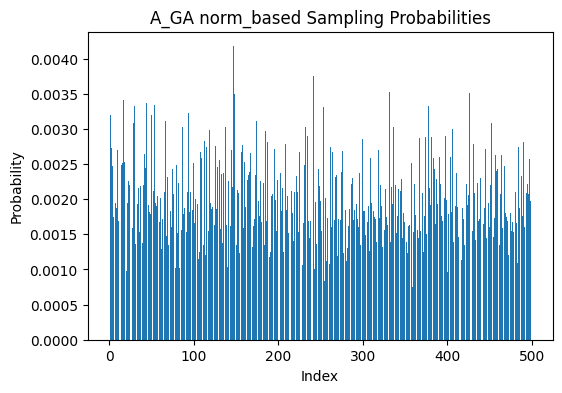
\includegraphics[width=0.5\textwidth]{/home/tagore/repos/STAT260/HW2/assets/Q9_A_GA norm_based Sampling Probabilities.png}
    \caption{GA Norm based probability distribution}
    \label{fig:GA_norm_based_prob}
\end{figure}

\begin{figure}[H]
    \centering
    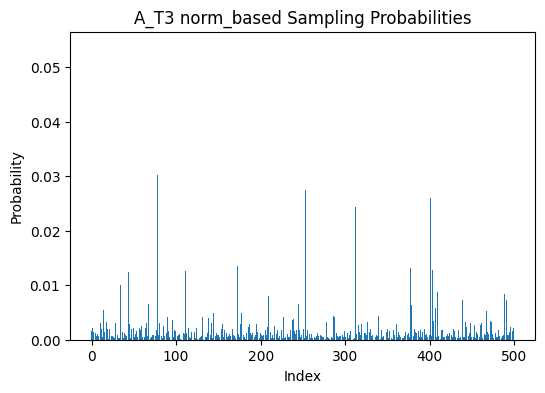
\includegraphics[width=0.5\textwidth]{/home/tagore/repos/STAT260/HW2/assets/Q9_A_T3 norm_based Sampling Probabilities.png}
    \caption{T3 Norm based probability distribution}
    \label{fig:T3_norm_based_prob}
\end{figure}

\begin{figure}[H]
    \centering
    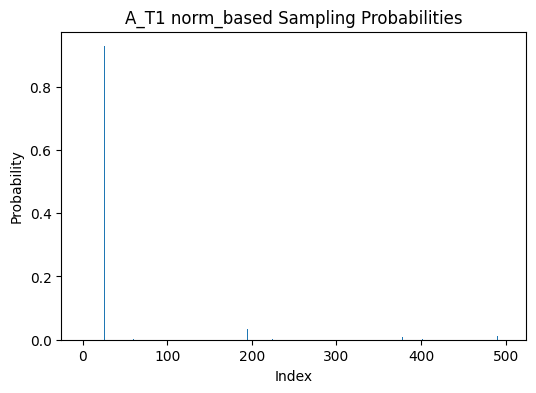
\includegraphics[width=0.5\textwidth]{/home/tagore/repos/STAT260/HW2/assets/Q9_A_T1 norm_based Sampling Probabilities.png}
    \caption{T1 Norm based probability distribution}
    \label{fig:T1_norm_based_prob}
\end{figure}

We will now plot the Frobenius and spectral error for the approximations of the three matrix multiplications.

\begin{figure}[H]
    \centering
    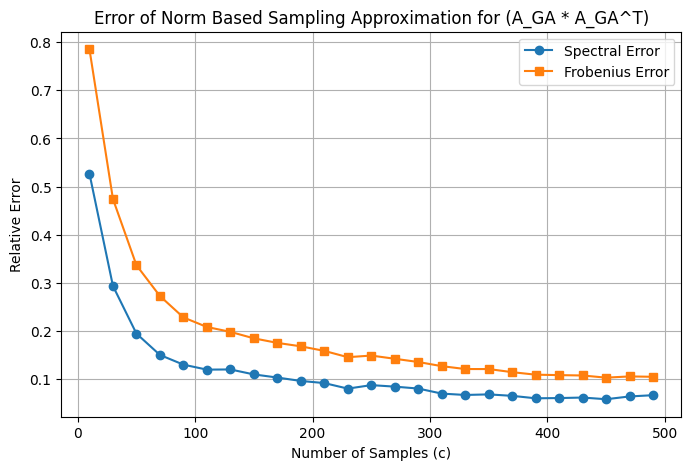
\includegraphics[width=0.5\textwidth]{/home/tagore/repos/STAT260/HW2/assets/Q9_Error of Norm Based Sampling Approximation for (A_GA * A_GA^T).png}
    \caption{Error of Norm Based Sampling Approximation for (\(A_{GA}^\top A_{GA}\))}
    \label{fig:GA_norm_based_error}
\end{figure}

\begin{figure}[H]
    \centering
    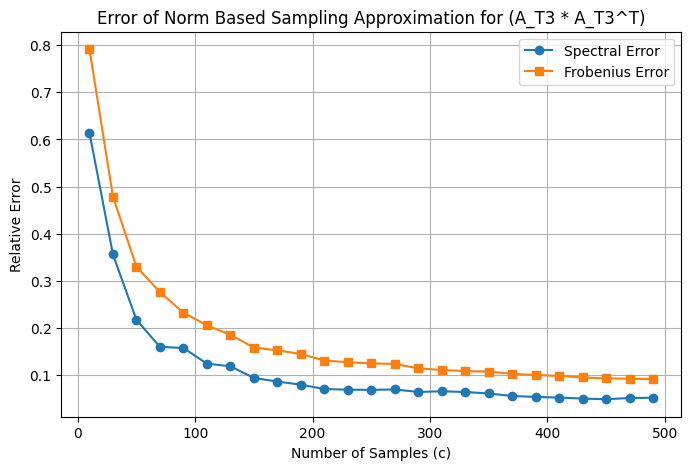
\includegraphics[width=0.5\textwidth]{/home/tagore/repos/STAT260/HW2/assets/Q9_Error of Norm Based Sampling Approximation for (A_T3 * A_T3^T).png}
    \caption{Error of Norm Based Sampling Approximation for (\(A_{T3}^\top A_{T3}\))}
    \label{fig:T3s_norm_based_error}
\end{figure}

\begin{figure}[H]
    \centering
    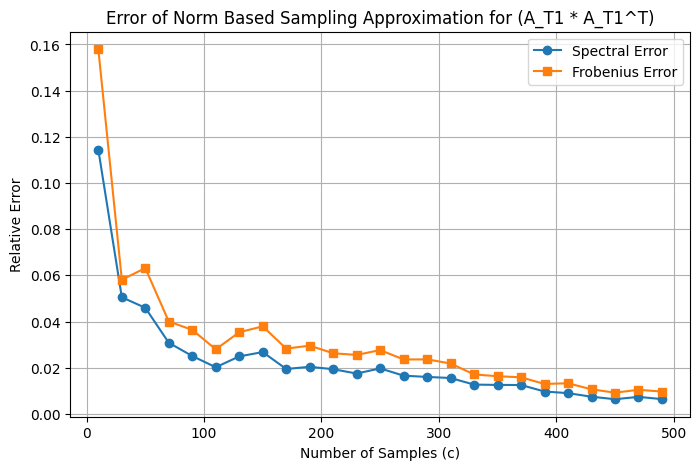
\includegraphics[width=0.5\textwidth]{/home/tagore/repos/STAT260/HW2/assets/Q_9_Error of Norm Based Sampling Approximation for (A_T1 * A_T1^T).png}
    \caption{Error of Norm Based Sampling Approximation for (\(A_{T1}^\top A_{T1}\))}
    \label{fig:T1_norm_based_error}
\end{figure}

\newpage

\section*{Problem 10}

We will now plot the Frobenius and spectral error for the approximations of the three left singular matrices multiplication.

\begin{figure}[H]
    \centering
    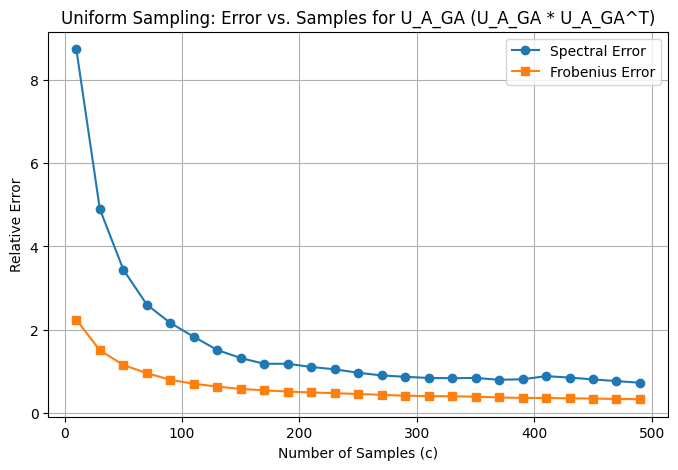
\includegraphics[width=0.5\textwidth]{/home/tagore/repos/STAT260/HW2/assets/Q10_Uniform Sampling: Error vs. Samples for U_A_GA (U_A_GA * U_A_GA^T).png}
    \caption{Error of Uniform Based Sampling Approximation for (\(U_{GA}^\top U_{GA}\))}
    \label{fig:GA_uniform_based_error}
\end{figure}

\begin{figure}[H]
    \centering
    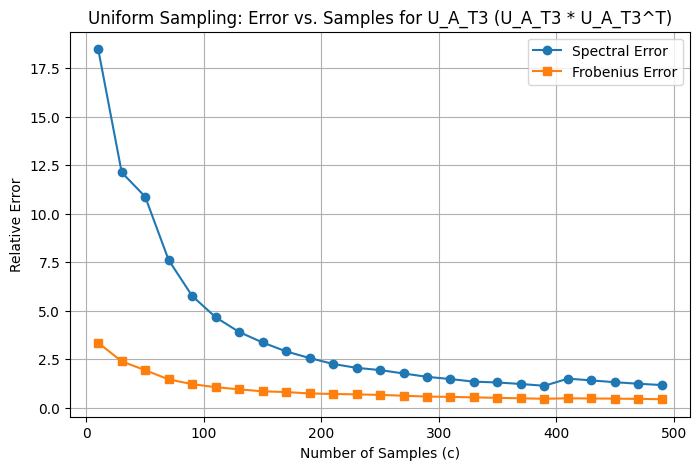
\includegraphics[width=0.5\textwidth]{/home/tagore/repos/STAT260/HW2/assets/Q10_Uniform Sampling: Error vs. Samples for U_A_T3 (U_A_T3 * U_A_T3^T).png}
    \caption{Error of Uniform Based Sampling Approximation for (\(U_{T3}^\top U_{T3}\))}
    \label{fig:T1_uniform_based_error}
\end{figure}

\begin{figure}[H]
    \centering
    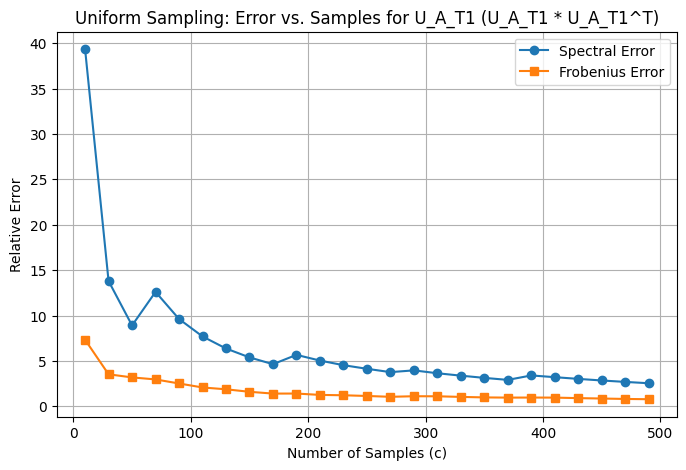
\includegraphics[width=0.5\textwidth]{/home/tagore/repos/STAT260/HW2/assets/Q10_Uniform Sampling: Error vs. Samples for U_A_T1 (U_A_T1 * U_A_T1^T).png}
    \caption{Error of Uniform Based Sampling Approximation for (\(U_{T1}^\top U_{T1}\))}
    \label{fig:T3_uniform_based_error}
\end{figure}

\newpage

\section*{Problem 11}

We will now plot the Frobenius and spectral error for the approximations of \(A^\top A\) using leverage score sampling.

\begin{figure}[H]
    \centering
    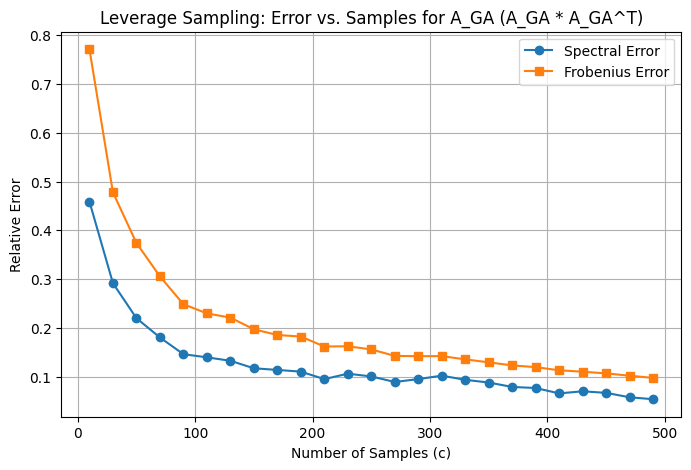
\includegraphics[width=0.5\textwidth]{/home/tagore/repos/STAT260/HW2/assets/Q11_Leverage Sampling: Error vs. Samples for A_GA (A_GA * A_GA^T).png}
    \caption{Error of Leverage Based Sampling Approximation for (\(A_{GA}^\top A_{GA}\))}
    \label{fig:GA_leverage_based_error}
\end{figure}

\begin{figure}[H]
    \centering
    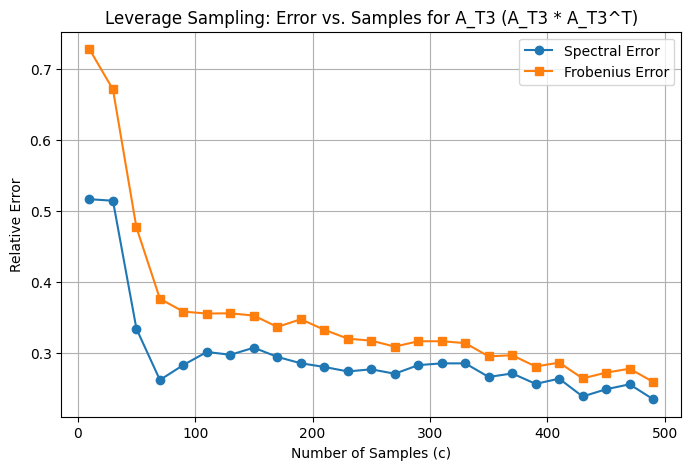
\includegraphics[width=0.5\textwidth]{/home/tagore/repos/STAT260/HW2/assets/Q11_Leverage Sampling: Error vs. Samples for A_T3 (A_T3 * A_T3^T).png}
    \caption{Error of Leverage Based Sampling Approximation for (\(A_{T3}^\top A_{T3}\))}
    \label{fig:T1_leverage_based_error}
\end{figure}

\begin{figure}[H]
    \centering
    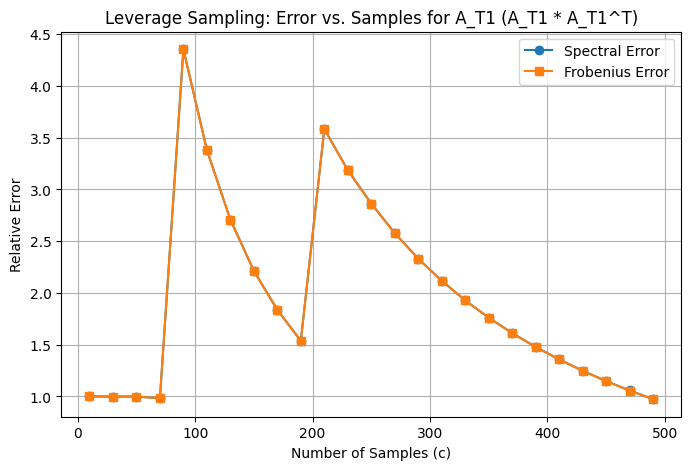
\includegraphics[width=0.5\textwidth]{/home/tagore/repos/STAT260/HW2/assets/Q11_Leverage Sampling: Error vs. Samples for A_T1 (A_T1 * A_T1^T).png}
    \caption{Error of Leverage Based Sampling Approximation for (\(A_{T1}^\top A_{T1}\))}
    \label{fig:T3_leverage_based_error}
\end{figure}

The results looks similar for $A_{GA}$ and $A_{T3}$, but the error for $A_{T1}$ is significantly higher than the other two matrices. 
This means that the leverage score sampling is not as effective for $A_{T1}$ as it is for the other two matrices.


\section*{Problem 12}

We will now plot the Frobenius and spectral error for the approximations of \(A A^\top\) using gaussian projection and $\{\pm 1\}$ projection.
\begin{figure}[H]
    \centering
    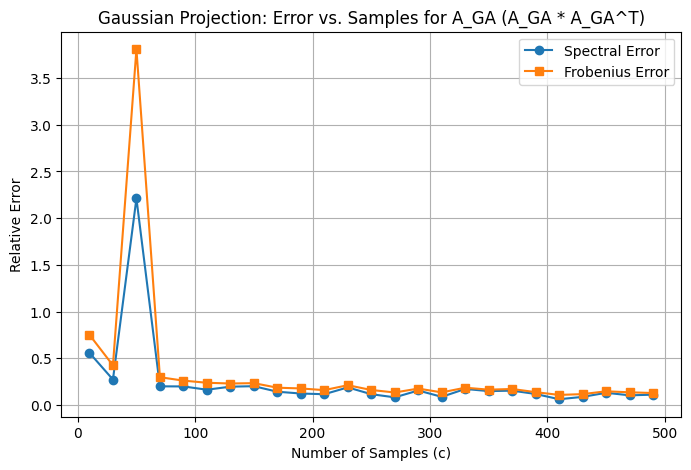
\includegraphics[width=0.5\textwidth]{/home/tagore/repos/STAT260/HW2/assets/Q12_Gaussian Projection: Error vs. Samples for A_GA (A_GA * A_GA^T).png}
    \caption{Error of Gaussian Projection Approximation for (\(A_{GA} A_{GA}^\top\))}
    \label{fig:GA_gaussian_projection_error}
\end{figure}
\begin{figure}[H]
    \centering
    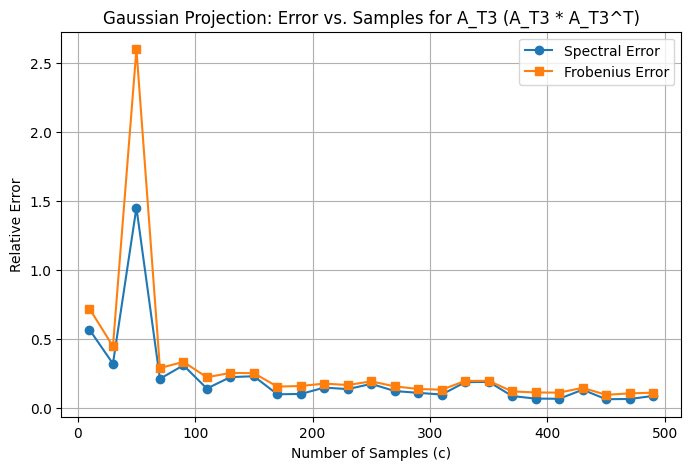
\includegraphics[width=0.5\textwidth]{/home/tagore/repos/STAT260/HW2/assets/Q12_Gaussian Projection: Error vs. Samples for A_T3 (A_T3 * A_T3^T).png}
    \caption{Error of Gaussian Projection Approximation for (\(A_{T3} A_{T3}^\top\))}
    \label{fig:T3_gaussian_projection_error}
\end{figure}

\begin{figure}[H]
    \centering
    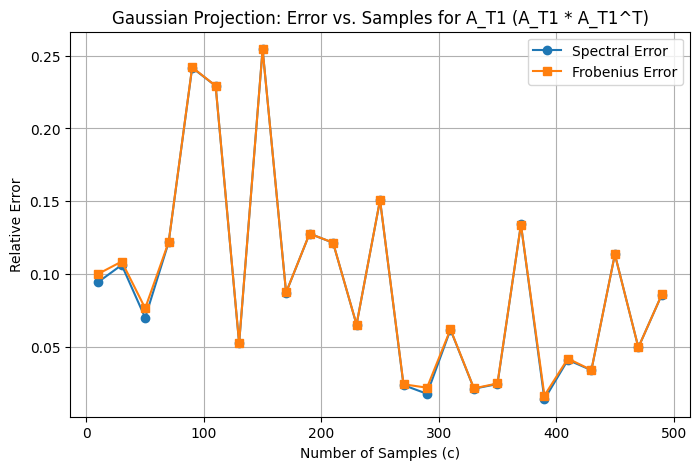
\includegraphics[width=0.5\textwidth]{/home/tagore/repos/STAT260/HW2/assets/Q12_Gaussian Projection: Error vs. Samples for A_T1 (A_T1 * A_T1^T).png}
    \caption{Error of Gaussian Projection Approximation for (\(A_{T1} A_{T1}^\top\))}
    \label{fig:T1_gaussian_projection_error}
\end{figure}

\begin{figure}[H]
    \centering
    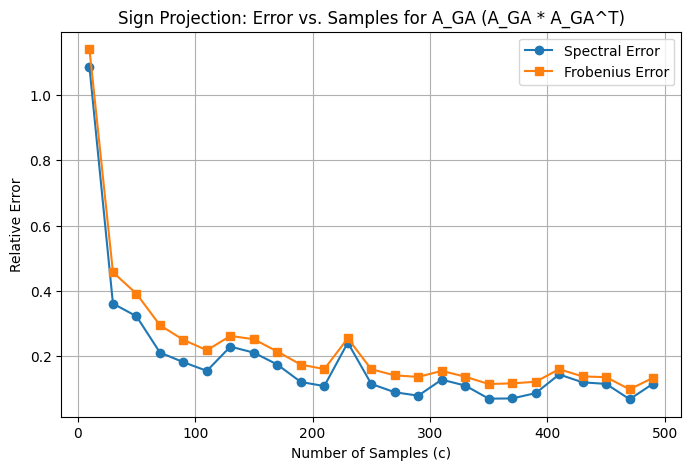
\includegraphics[width=0.5\textwidth]{/home/tagore/repos/STAT260/HW2/assets/Q12_Sign Projection: Error vs. Samples for A_GA (A_GA * A_GA^T).png}
    \caption{Error of $\{\pm 1\}$ Projection Approximation for (\(A_{GA} A_{GA}^\top\))}
    \label{fig:GA_pm1_projection_error}
\end{figure}

\begin{figure}[H]
    \centering
    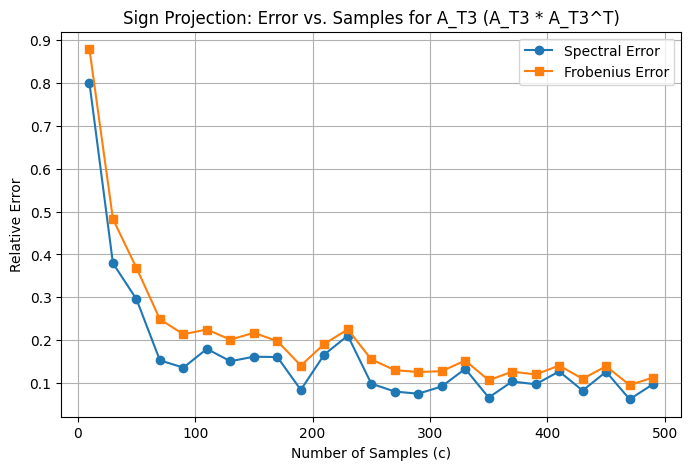
\includegraphics[width=0.5\textwidth]{/home/tagore/repos/STAT260/HW2/assets/Q12_Sign Projection: Error vs. Samples for A_T3 (A_T3 * A_T3^T).png}
    \caption{Error of $\{\pm 1\}$ Projection Approximation for (\(A_{T3} A_{T3}^\top\))}
    \label{fig:T3_pm1_projection_error}
\end{figure}\

\begin{figure}[H]
    \centering
    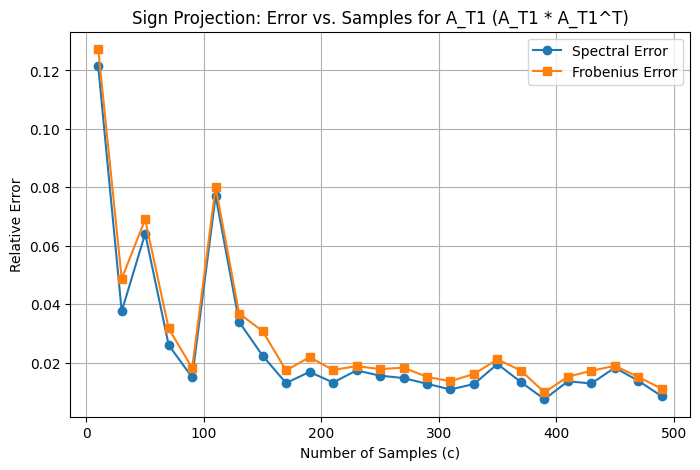
\includegraphics[width=0.5\textwidth]{/home/tagore/repos/STAT260/HW2/assets/Q12_Sign Projection: Error vs. Samples for A_T1 (A_T1 * A_T1^T).png}
    \caption{Error of $\{\pm 1\}$ Projection Approximation for (\(A_{T1} A_{T1}^\top\))}
    \label{fig:T1_pm1_projection_error}
\end{figure}

Comparing the results of the Gaussian projection and $\{\pm 1\}$ projection: The gaussian projection produces more stable results and has slightly smaller error for projecting $A_{GA}$ and $A_{T3}$ when there is reasonbale amount of dimensions. 
The guassian projection performs extremelly well for $A_{T1}$, while the $\{\pm 1\}$ projection has a higher error for all three matrices. The only extreme case is that sign projection seems to outperform gaussian projection for $A_{T1}$ when the number of dimensions is small.

Comparing the results of projection and sampling: The projection method has much lower error compare to uniform sampling and overall slight lower error when comparing to norm based sampling and leverage score sampling. The projection method is more stable and has lower error for all three matrices.
However, there are times where the projection method shows outlier errors, such as the gaussian projection for $A_{GA}$ when the number of dimensions is small.

\section*{Problem 13}

We will now plot 3D plot of the error of the sparse approximations of \(A A^\top\) using gaussian projection and $\{\pm 1\}$ projection. The two axes are the sparsity and the number of dimensions, and the third axis is the error.

\begin{figure}[H]
    \centering
    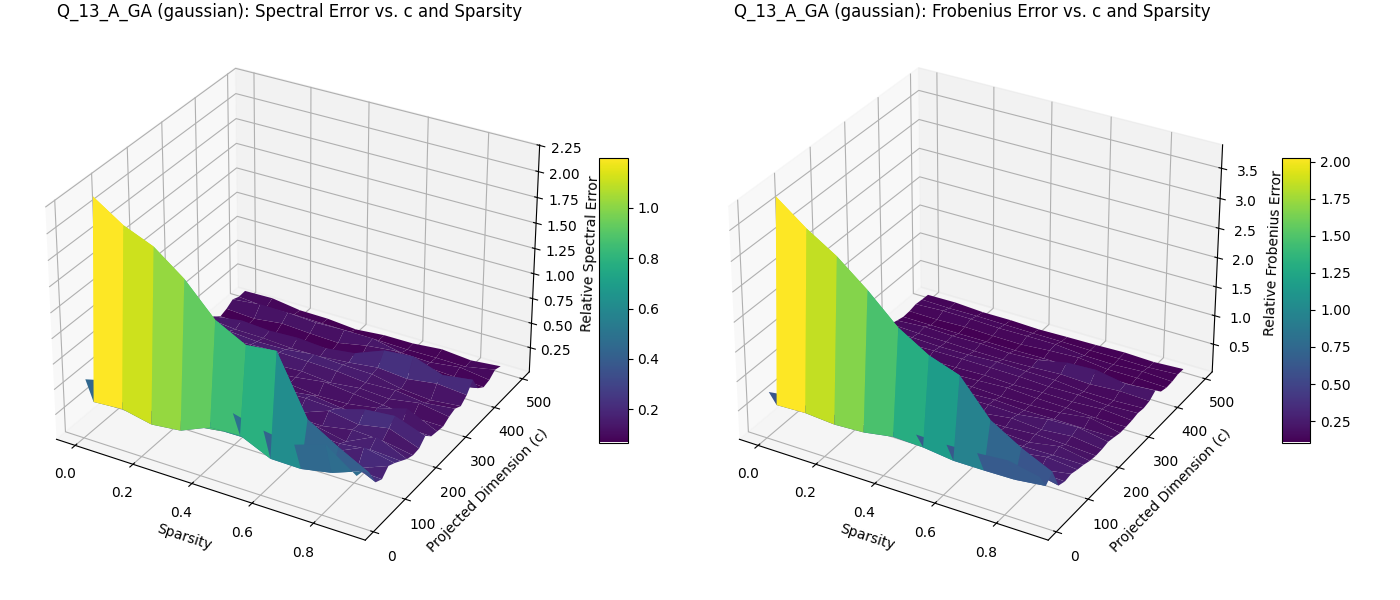
\includegraphics[width=1\textwidth]{/home/tagore/repos/STAT260/HW2/assets/Q_13_A_GA_gaussian_errors.png}
    \caption{Error of Gaussian Projection Approximation for (\(A_{GA} A_{GA}^\top\))}
    \label{fig:GA_gaussian_projection_error_3d}
\end{figure}

\begin{figure}[H]
    \centering
    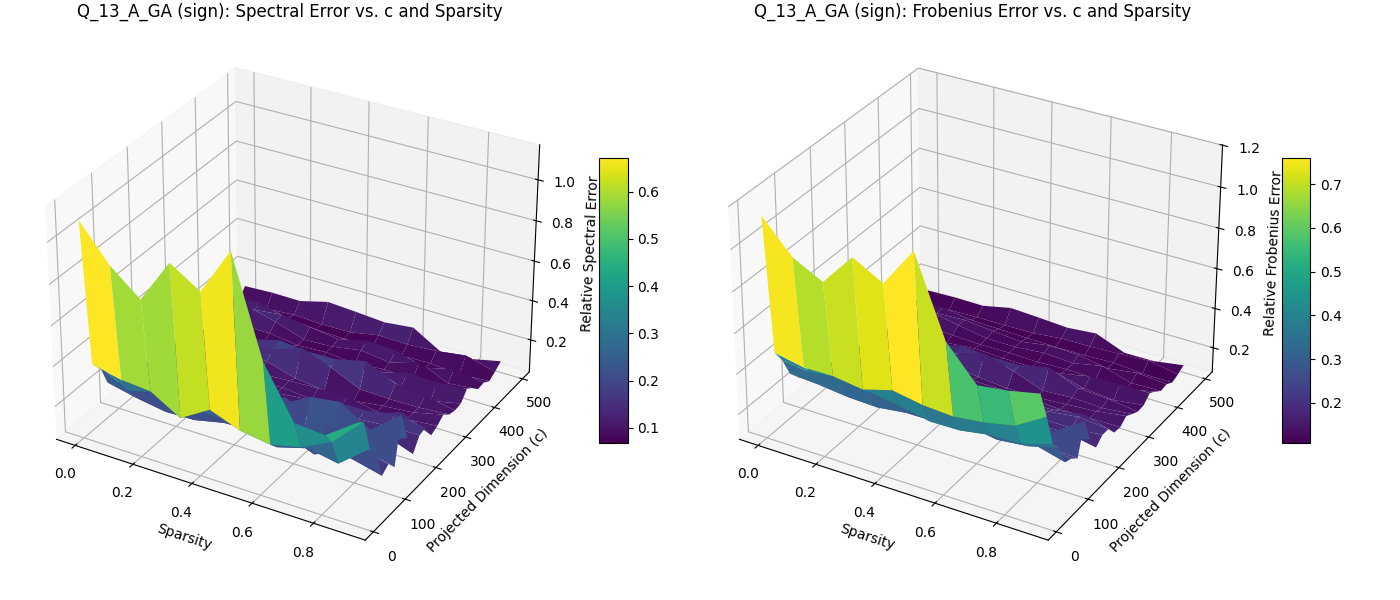
\includegraphics[width=1\textwidth]{/home/tagore/repos/STAT260/HW2/assets/Q_13_A_GA_sign_errors.png}
    \caption{Error of $\{\pm 1\}$ Projection Approximation for (\(A_{GA} A_{GA}^\top\))}
    \label{fig:GA_pm1_projection_error_3d}
\end{figure}

\begin{figure}[H]
    \centering
    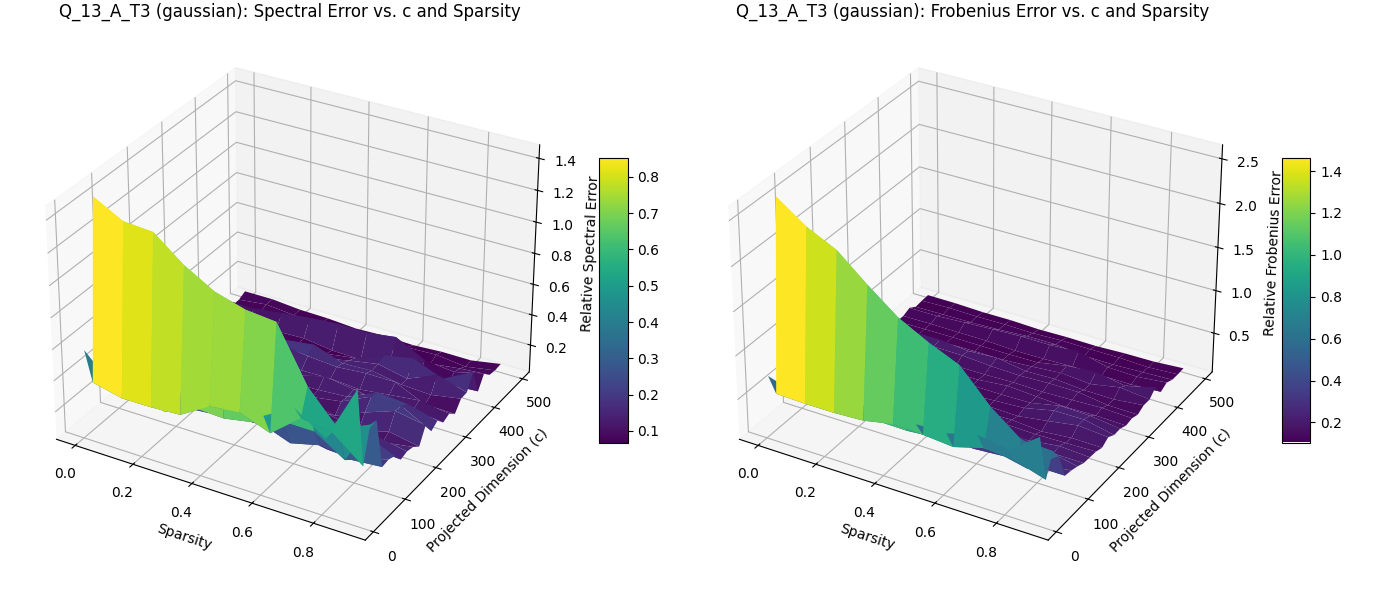
\includegraphics[width=1\textwidth]{/home/tagore/repos/STAT260/HW2/assets/Q_13_A_T3_gaussian_errors.png}
    \caption{Error of Gaussian Projection Approximation for (\(A_{T3} A_{T3}^\top\))}
    \label{fig:T3_gaussian_projection_error_3d}
\end{figure}

\begin{figure}[H]
    \centering
    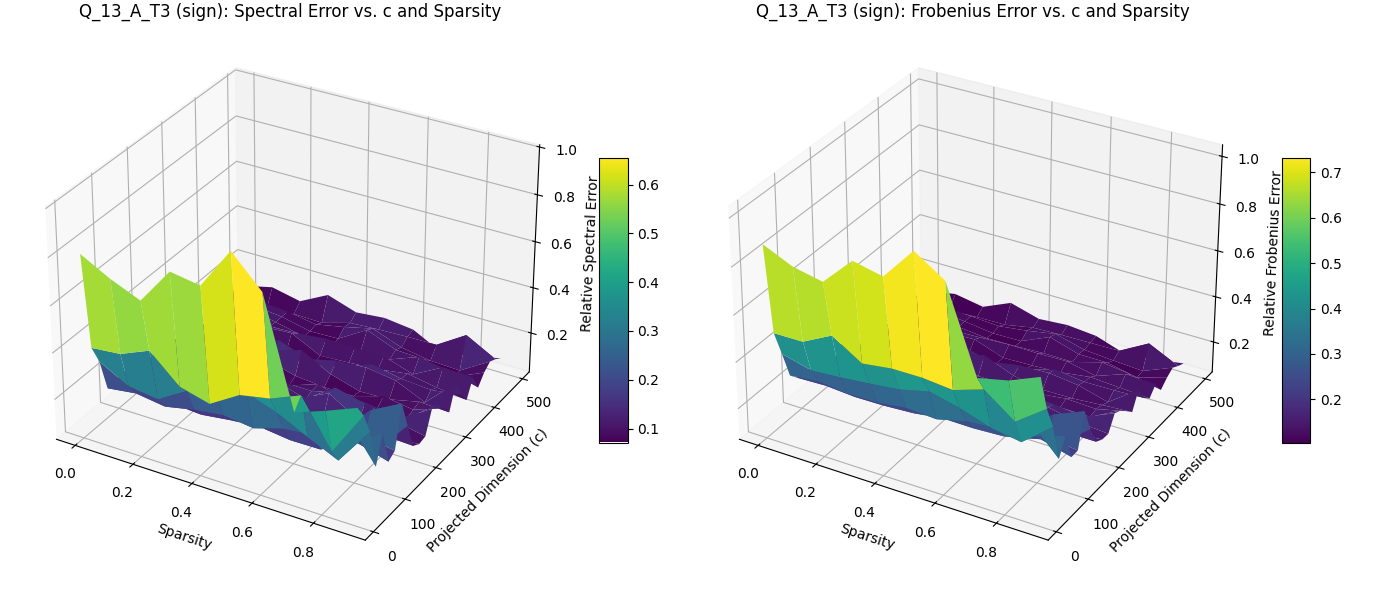
\includegraphics[width=1\textwidth]{/home/tagore/repos/STAT260/HW2/assets/Q_13_A_T3_sign_errors.png}
    \caption{Error of $\{\pm 1\}$ Projection Approximation for (\(A_{T3} A_{T3}^\top\))}
    \label{fig:T3_pm1_projection_error_3d}
\end{figure}

\begin{figure}[H]
    \centering
    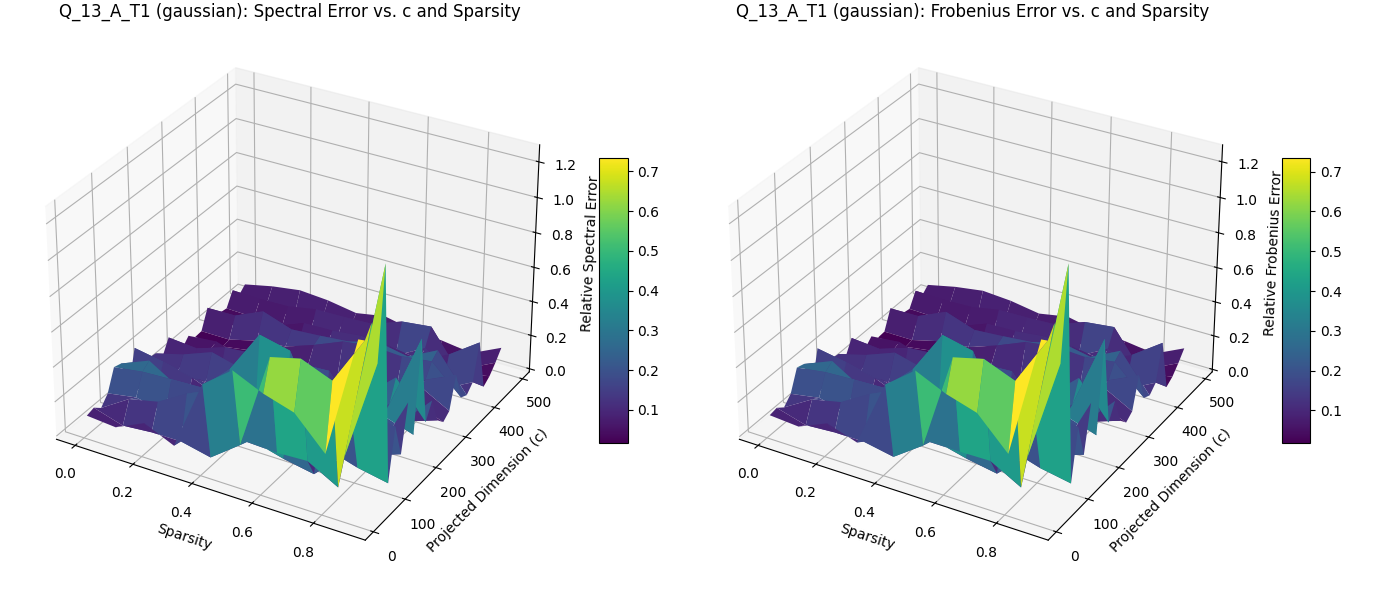
\includegraphics[width=1\textwidth]{/home/tagore/repos/STAT260/HW2/assets/Q_13_A_T1_gaussian_errors.png}
    \caption{Error of Gaussian Projection Approximation for (\(A_{T1} A_{T1}^\top\))}
    \label{fig:T1_gaussian_projection_error_3d}
\end{figure}
 
\begin{figure}[H]
    \centering
    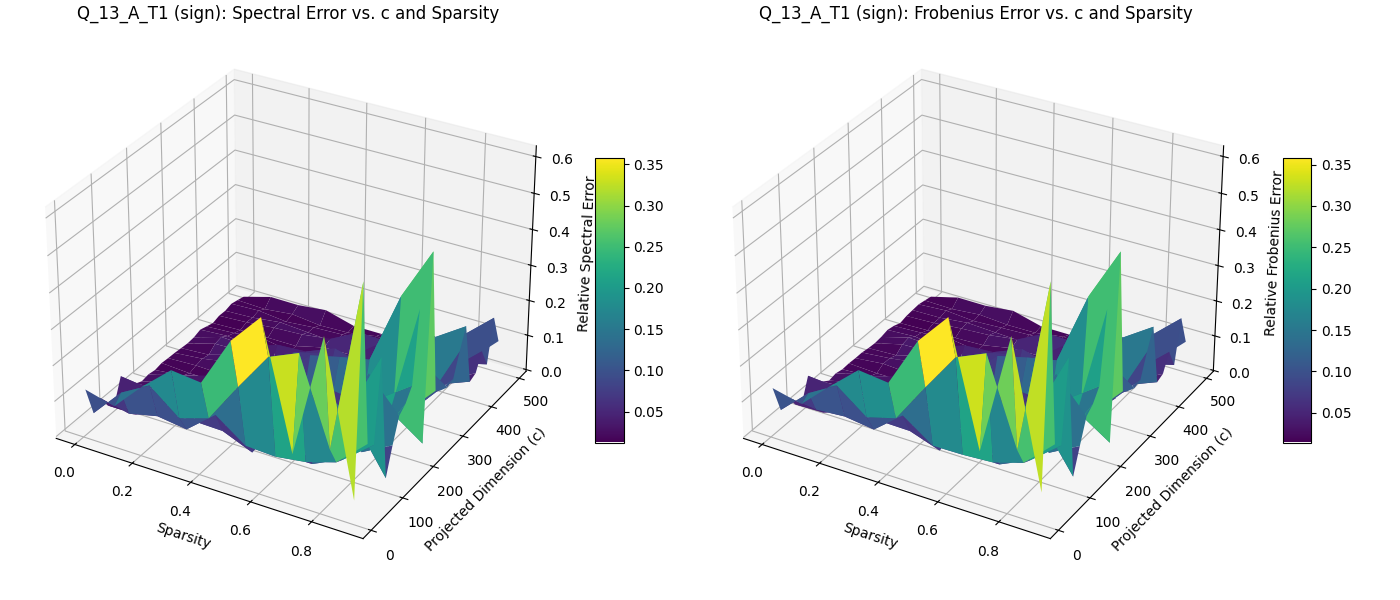
\includegraphics[width=1\textwidth]{/home/tagore/repos/STAT260/HW2/assets/Q_13_A_T1_sign_errors.png}
    \caption{Error of $\{\pm 1\}$ Projection Approximation for (\(A_{T1} A_{T1}^\top\))}
    \label{fig:T1_pm1_projection_error_3d}
\end{figure}

Both Gaussian projection and $\{\pm 1\}$ projection have similar error patterns for all three matrices. For $A_{GA}$ and $A_{T3}$, the error is relatively stable and low when the number of dimensions is large. 
In addition, both projection seems to perform well as we increase sparsity. However, for $A_{T1}$, the error is significantly higher than the other two matrices, and the error is not as stable as the other two matrices.
For both projection, the errors are higher when the sparsity is high, and the errors are more unstable when the sparsity is high.


\section*{Problem 13.5 Variability Analysis}
\subsection*{\(A_{GA}\)}

\begin{figure}[H]
    \centering
    % Frobenius Error Comparison
    \begin{subfigure}[b]{0.48\textwidth}
        \centering
        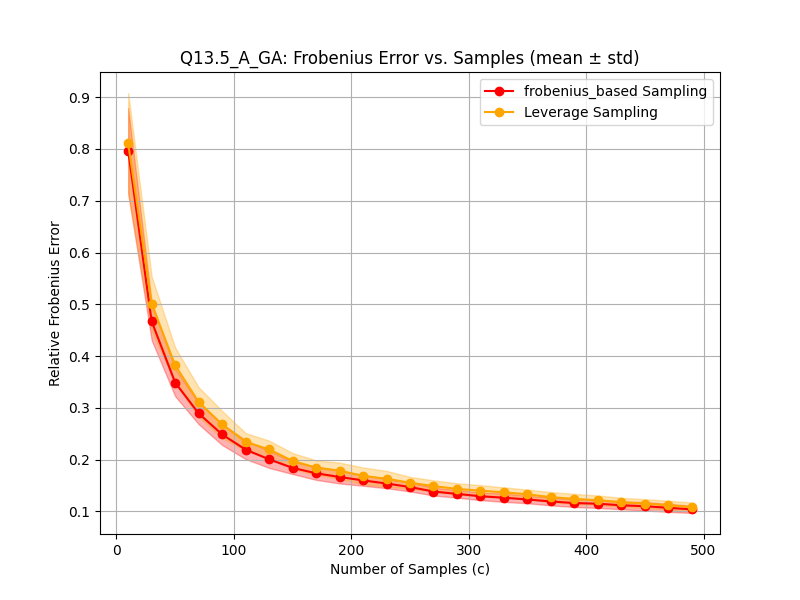
\includegraphics[width=\textwidth]{/home/tagore/repos/STAT260/HW2/assets/Q13.5_A_GA_frobenius_error.png}
        \caption{Sampling: Frobenius Error}
        \label{fig:GA_fs}
    \end{subfigure}
    \hfill
    \begin{subfigure}[b]{0.48\textwidth}
        \centering
        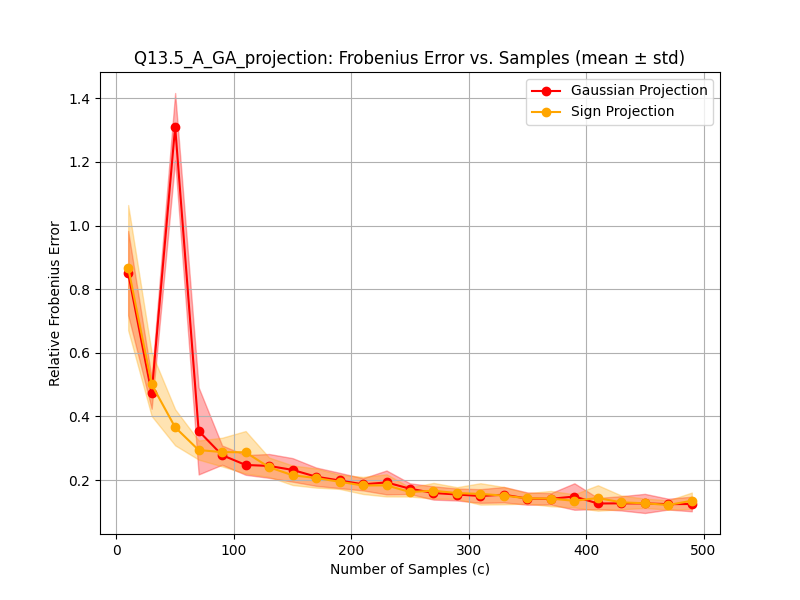
\includegraphics[width=\textwidth]{/home/tagore/repos/STAT260/HW2/assets/Q13.5_A_GA_projection_frobenius_error.png}
        \caption{Projection: Frobenius Error}
        \label{fig:GA_fp}
    \end{subfigure}
    
    \vspace{0.5cm}
    
    % Spectral Error Comparison
    \begin{subfigure}[b]{0.48\textwidth}
        \centering
        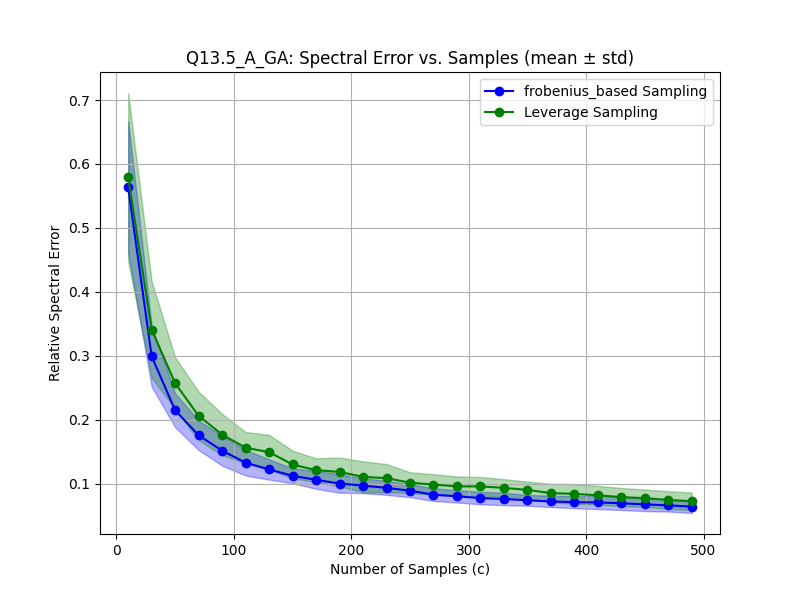
\includegraphics[width=\textwidth]{/home/tagore/repos/STAT260/HW2/assets/Q13.5_A_GA_spectral_error.png}
        \caption{Sampling: Spectral Error}
        \label{fig:GA_ss}
    \end{subfigure}
    \hfill
    \begin{subfigure}[b]{0.48\textwidth}
        \centering
        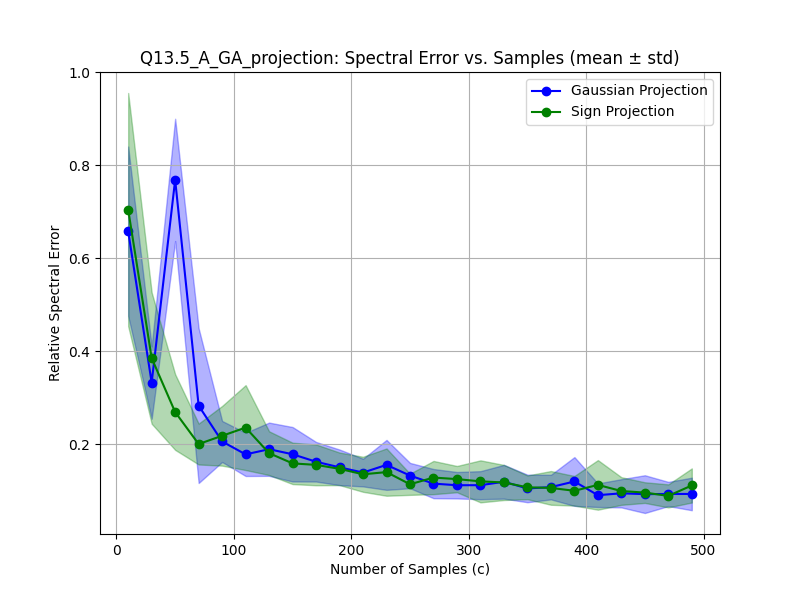
\includegraphics[width=\textwidth]{/home/tagore/repos/STAT260/HW2/assets/Q13.5_A_GA_projection_spectral_error.png}
        \caption{Projection: Spectral Error}
        \label{fig:GA_sp}
    \end{subfigure}
    
    \caption{\(A_{GA}\): Comparison of Random Sampling and Random Projection}
    \label{fig:GA_comparison}
\end{figure}

\newpage
\subsection*{\(A_{T1}\)}

\begin{figure}[H]
    \centering
    % Frobenius Error Comparison
    \begin{subfigure}[b]{0.48\textwidth}
        \centering
        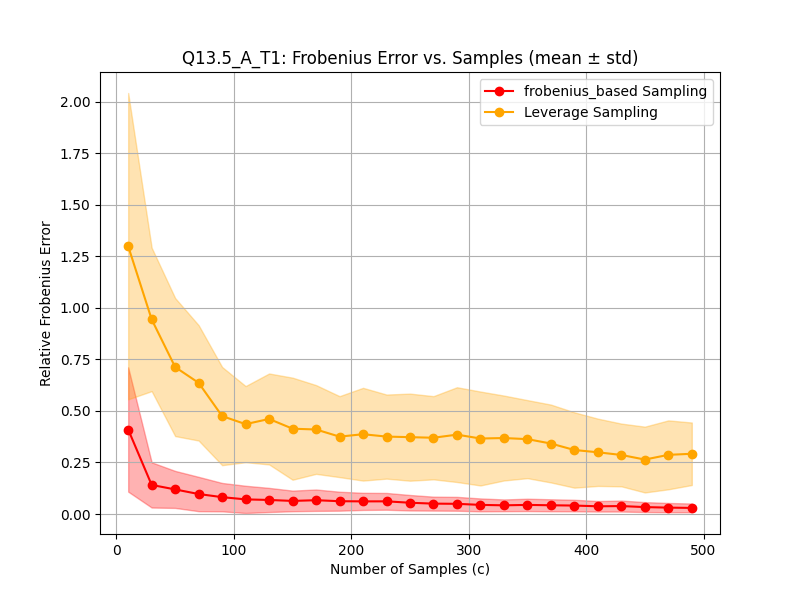
\includegraphics[width=\textwidth]{/home/tagore/repos/STAT260/HW2/assets/Q13.5_A_T1_frobenius_error.png}
        \caption{Sampling: Frobenius Error}
        \label{fig:T1_fs}
    \end{subfigure}
    \hfill
    \begin{subfigure}[b]{0.48\textwidth}
        \centering
        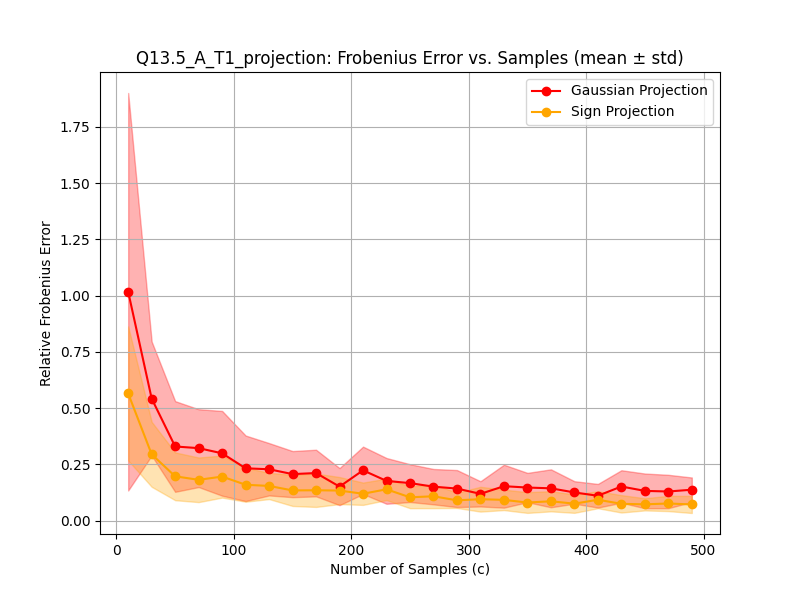
\includegraphics[width=\textwidth]{/home/tagore/repos/STAT260/HW2/assets/Q13.5_A_T1_projection_frobenius_error.png}
        \caption{Projection: Frobenius Error}
        \label{fig:T1_fp}
    \end{subfigure}
    
    \vspace{0.5cm}
    
    % Spectral Error Comparison
    \begin{subfigure}[b]{0.48\textwidth}
        \centering
        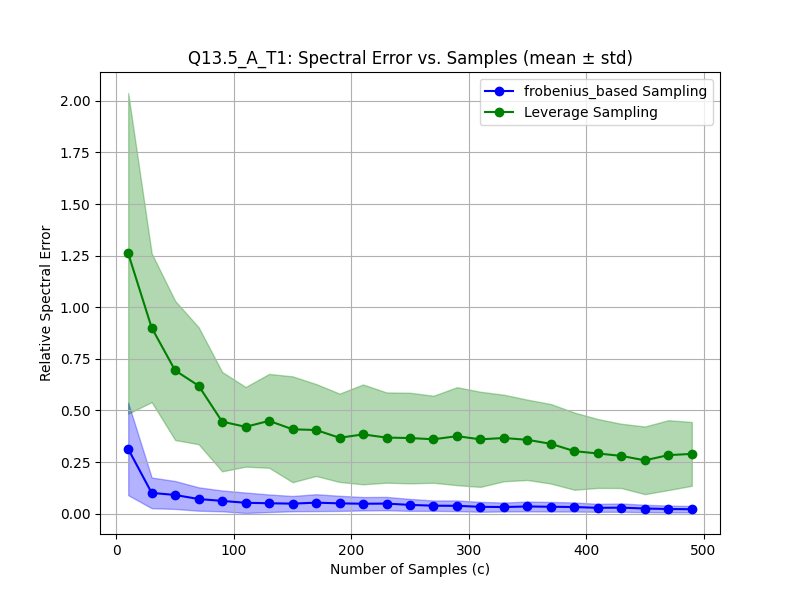
\includegraphics[width=\textwidth]{/home/tagore/repos/STAT260/HW2/assets/Q13.5_A_T1_spectral_error.png}
        \caption{Sampling: Spectral Error}
        \label{fig:T1_ss}
    \end{subfigure}
    \hfill
    \begin{subfigure}[b]{0.48\textwidth}
        \centering
        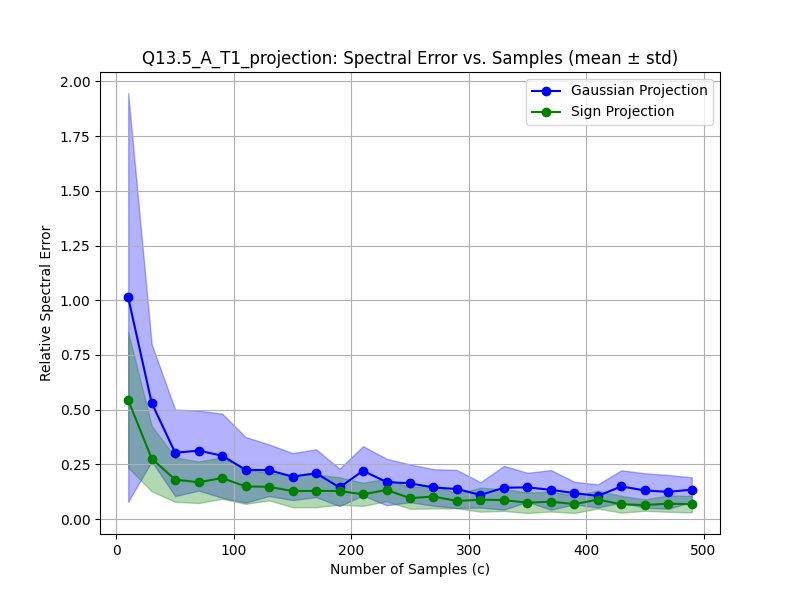
\includegraphics[width=\textwidth]{/home/tagore/repos/STAT260/HW2/assets/Q13.5_A_T1_projection_spectral_error.png}
        \caption{Projection: Spectral Error}
        \label{fig:T1_sp}
    \end{subfigure}
    
    \caption{\(A_{T1}\): Comparison of Random Sampling and Random Projection}
    \label{fig:T1_comparison}
\end{figure}

\newpage
\subsection*{\(A_{T3}\)}

\begin{figure}[H]
    \centering
    % Frobenius Error Comparison
    \begin{subfigure}[b]{0.48\textwidth}
        \centering
        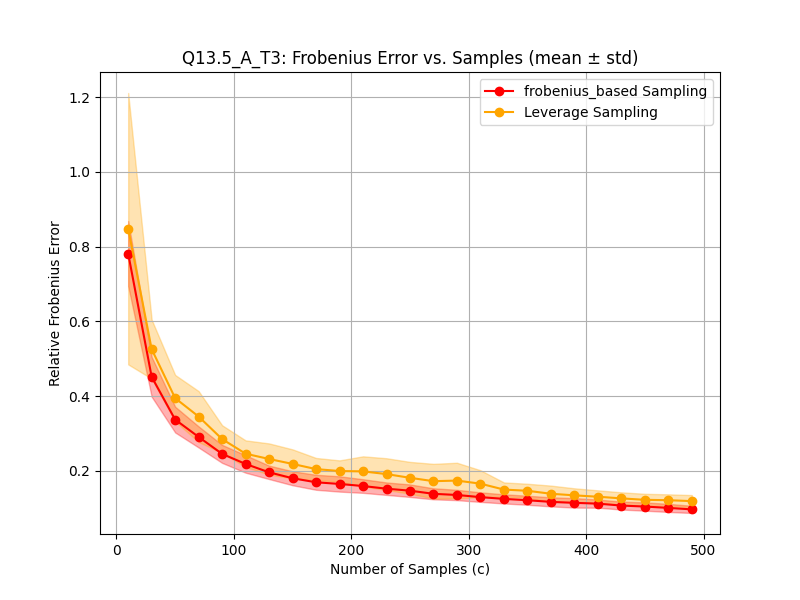
\includegraphics[width=\textwidth]{/home/tagore/repos/STAT260/HW2/assets/Q13.5_A_T3_frobenius_error.png}
        \caption{Sampling: Frobenius Error}
        \label{fig:T3_fs}
    \end{subfigure}
    \hfill
    \begin{subfigure}[b]{0.48\textwidth}
        \centering
        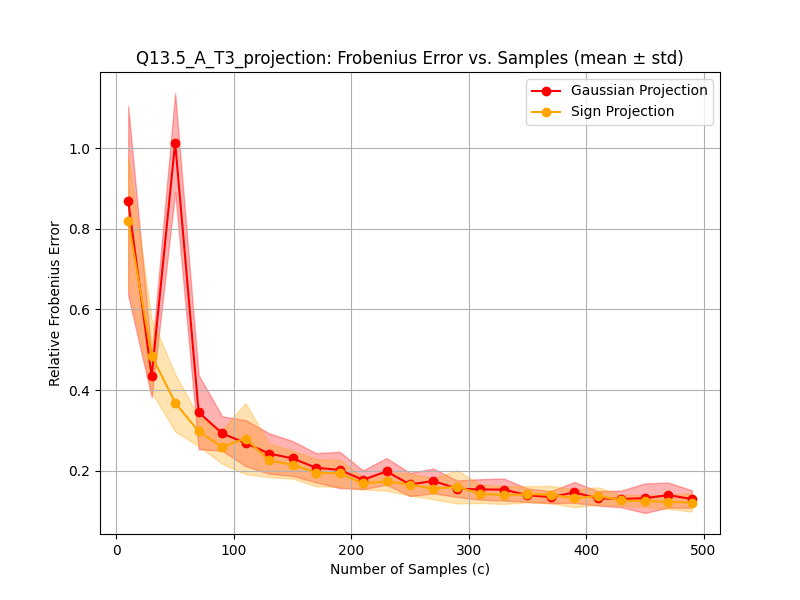
\includegraphics[width=\textwidth]{/home/tagore/repos/STAT260/HW2/assets/Q13.5_A_T3_projection_frobenius_error.png}
        \caption{Projection: Frobenius Error}
        \label{fig:T3_fp}
    \end{subfigure}
    
    \vspace{0.5cm}
    
    % Spectral Error Comparison
    \begin{subfigure}[b]{0.48\textwidth}
        \centering
        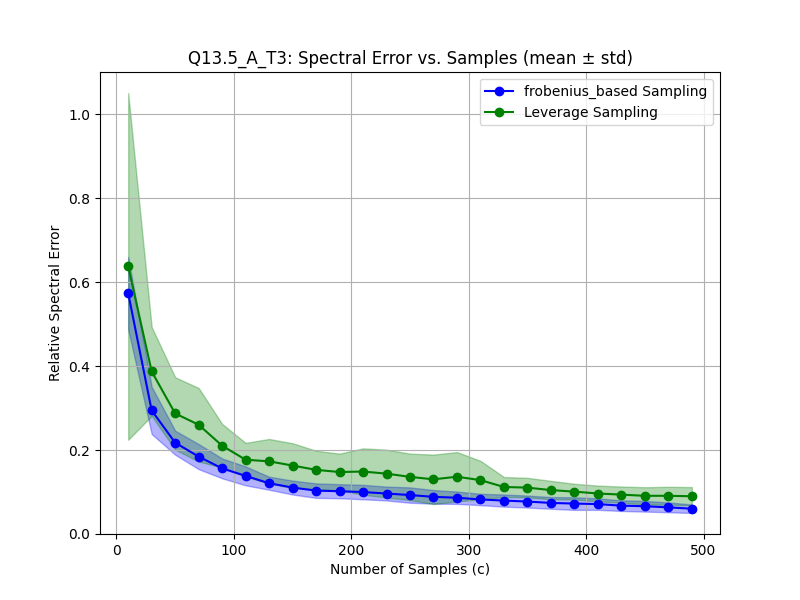
\includegraphics[width=\textwidth]{/home/tagore/repos/STAT260/HW2/assets/Q13.5_A_T3_spectral_error.png}
        \caption{Sampling: Spectral Error}
        \label{fig:T3_ss}
    \end{subfigure}
    \hfill
    \begin{subfigure}[b]{0.48\textwidth}
        \centering
        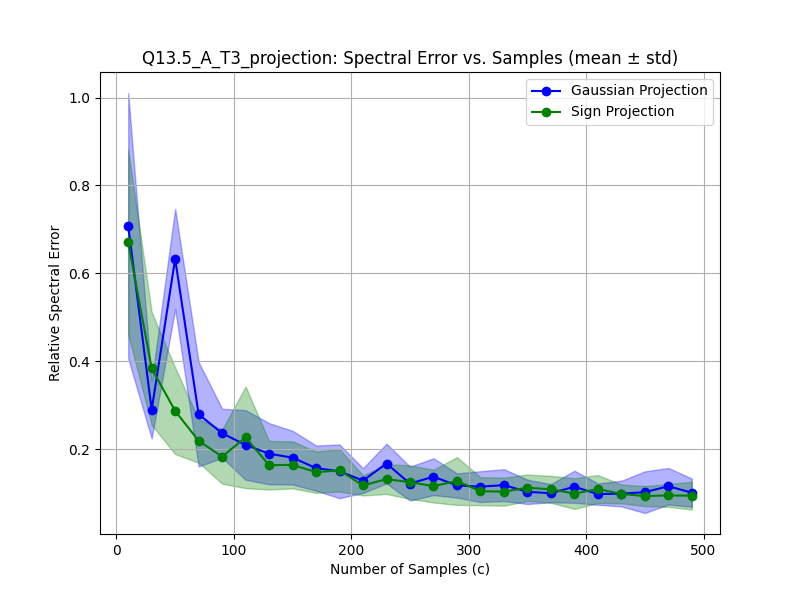
\includegraphics[width=\textwidth]{/home/tagore/repos/STAT260/HW2/assets/Q13.5_A_T3_projection_spectral_error.png}
        \caption{Projection: Spectral Error}
        \label{fig:T3_sp}
    \end{subfigure}
    
    \caption{\(A_{T3}\): Comparison of Random Sampling and Random Projection}
    \label{fig:T3_comparison}
\end{figure}





% \section*{Problem 2}
% Here is an example of a graph:
% \begin{figure}[h!]
%     \centering
%     \includegraphics[width=0.5\textwidth]{example-graph.png}
%     \caption{Example Graph}
%     \label{fig:example-graph}
% \end{figure}

\end{document}